\documentclass[a4paper,11pt]{article}
\usepackage{jheppub} % for details on the use of the package, please see the JINST-author-manual
\usepackage{lineno}
%\linenumbers
\usepackage{cmupint}
%packages I added after the fact
\usepackage{graphicx} % Required for inserting images
%\usepackage[utf8]{inputenc}
\usepackage[T1]{fontenc}
\usepackage{amsmath}
\usepackage{graphicx}
\usepackage{latexsym,amssymb,lmodern}
\usepackage{float}
\usepackage[colorinlistoftodos]{todonotes}
%\usepackage[a4paper,top=2cm,bottom=2cm,left=2cm,right=2cm,marginparwidth=1.75cm]{geometry}
\usepackage{hyperref}
\usepackage{xcolor}
\usepackage{soul}
\usepackage{cancel}
\usepackage{appendix}
\newtheorem{definition}{Definition}
\newtheorem{theorem}{Theorem}
%\newtheorem{question}{Question}
\newtheorem{importantrelation}{Important Relation}
\newtheorem{question}{Question}
\newcommand{\normord}[1]{:\mathrel{#1}:}
\usepackage{wrapfig}
\usepackage{braket}
\usepackage{physics}
\usepackage{ulem}
\usepackage{cancel}
\usepackage{comment}
%\usepackage{parskip}
%\setlength\parindent{24pt}
\usepackage{enumitem}
%\usepackage{titling}
\usepackage{slashed}
\usepackage{mathscinet}
\usepackage{dsfont} 
\usepackage{simpler-wick}
\usepackage{tikz}
%\usepackage{tikz-feynman}
\usepackage[compat=1.1.0]{tikz-feynman}
%stuff needed to input the github logo
\usepackage{fontawesome5}
\usepackage{xspace}
\usepackage{epigraph}
%\usepackage{fixltx2e}

\makeatletter
\newcommand{\github}[1]{%
   \href{#1}{\faGithubSquare}%
}
\makeatother

%Feynman rule for graviton propagator/legs
\tikzset{graviton/.style={decorate, decoration={snake, amplitude=.4mm, segment length=1.5mm, pre length=.5mm, post length=.5mm}, double}}

\definecolor{green3}{RGB}{44,160,44}

\newcommand{\ac}[1]{\textcolor{green3}{[\textbf{AC:}] #1}}

%\arxivnumber{1234.56789} % if you have one

\title{Everything S-Matrix}

% Collaborations

\author[a]{Alexander Cassem}
\affiliation[a]{Institute of Cosmology, Tufts University, Medford, MA 02155, USA}

% E-mail addresses: only for the corresponding author
\emailAdd{alexander.cassem@tufts.edu}


\abstract{
These are personal notes written in the style of ``lecture notes'' as a way to help organize in my own mind the various topics associated with the S-matrix. These notes are a WORK IN PROGRESS and are not meant to be any definitive source material on the various subjects found within. Please check any results for yourself, as well as the cited source material. 
}



\begin{document}
\maketitle
\flushbottom

\section{A Guide on the Literature}

\ac{Fill-in later, but briefly: trust chapters 1 and 4 of Eden's et al. textbook, and start with Mizera's notes since they are amazing} \cite{Eden:1966dnq,Mizera:2023tfe}.

\section{General Properties of Amplitudes}

\epigraph{The best assumptions are the ones you can't prove.}{\textit{Xi Yin}\\PHY253b}

The title of the section should really be ``\textit{Some} General Properties of Amplitudes,'' since the vastness of the literature on S-matrix results is staggering and ever changing. However, the core results from the 60's and 70's, being re-discovered and re-formulated will never change (only the efficiency of their derivation will). It is these core results that we will be looking at in this section by taking examples of physical setups that can be extended to a more general case. 

\subsection{Examples: $2\rightarrow 2$ Scattering of Identical Massless Scalars}

Consider the $2\rightarrow 2$ scattering amplitude of identical massive scalar particles. The $s$- and $t$-channel can be written in terms of the scattering angle $\theta$ as
\begin{equation}
    s = E^2 = 4(k^2+m^2)\:\:\text{and}\:\: t = -2k^2(1-\cos(\theta))\label{parameterization of s and t channels}.
\end{equation}
We know that the amplitude $A(s,t)$ can be analytically continued away from the physical region $s,t\in\mathbb{R}$ with $s\geq 4m^2-t$ with $t\leq 0$ \footnote{We will still denote the ampliude $\mathcal{A}(s,t)$}. Consider fixing $t<0$ and analytically continue $s$ into the complex plane. This can be see in figure \ref{Complex graph of s}.

\begin{figure}[h]
    \centering
    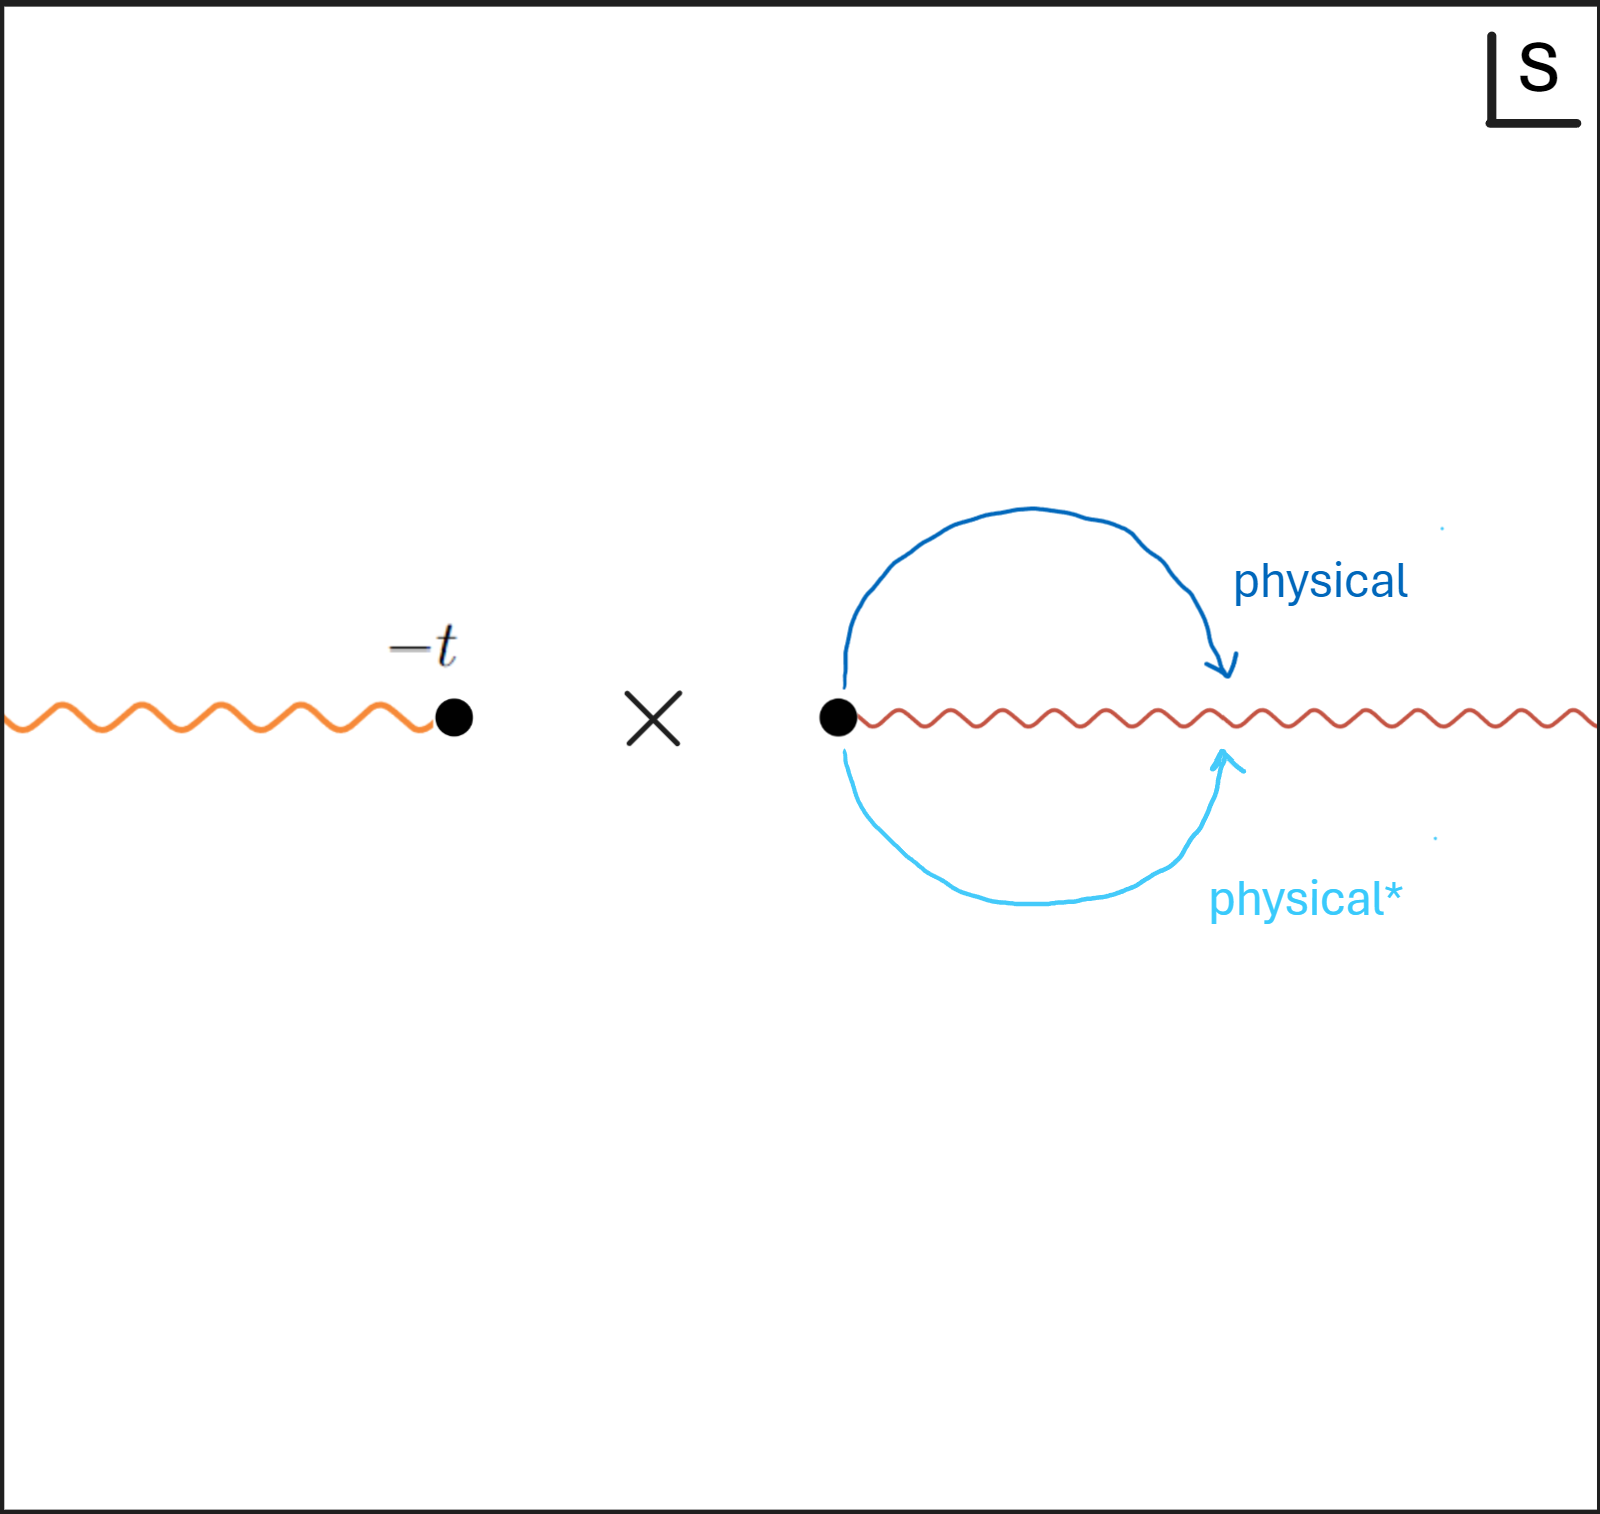
\includegraphics[width=0.5\linewidth]{s channel graph.png}
    \caption{Complex graph of $s$ with branch cuts on $s$-channel and $u$-channel with possible bound state poles denoted as x's.}
    \label{Complex graph of s}
\end{figure}
The \textit{branch cut} on the complex graph of $s$ denotes all the physical states of the theory based on the bounds of $s$. The physical amplitude can be written as
\begin{equation}
    \text{physical amplitude} = \lim_{\epsilon\rightarrow 0^+}A(s+i\epsilon,t)\label{physical amplitude}.
\end{equation}
The limit of \eqref{physical amplitude} is taken such that we analytically continue from above towards the branch cut. If we instead went from $0^-$, then we would have analytically continued from below, finding the complex conjugate of the physical amplitude. Analytically continuing the amplitude $A(s,t)$ is expected to obey the \textit{real analyticity} condition
\begin{equation}
    A(s^*,t^*) = (A(s,t))^*\label{reality condition},
\end{equation}
which can also be thought of as a reality condition \footnote{In perturbation theory,this follows from the reality of coupling constants in the Lagrangian.}. This is the first assumption we will make about the amplitude. The graph in \ref{Complex graph of s} of the $s$-channel is on the \textit{first Riemann sheet} or the \textit{physical sheet}. The cut on the LHS is a $u$-channel cut that starts at $-t$. The crosses denote possible bound state poles. The resonance poles are heinding on the \textit{second sheet} which can be found by translating between momentum to energy \footnote{A classical example from quantum mechanics is when graphing complex $p$ and finding the second sheet by using $p^2/2m = E\implies p = \pm i\sqrt{-2mE}$.}. 

The second assumption we make about the amplitude $A(s,t)$ is that it has a \textit{crossing symmetry}. Crossing symmetry, in terms of the channels, relates the different scattering channels $s,t$, and $u$ to each other via analytically continuing to different regions of $s,t$, and $u$. \ac{Insert Mandelstam graph from \cite{Eden:1966dnq}}. Note that all of the assumptions being made about $A(s,t)$ hold non-perturbatively. 

The third assumption we shall make is about unitarity. Remember that in the partial wave basis
\begin{equation}
    A(s,t) =16\pi i\sqrt{\frac{s}{s-4m^2}}\sum_{\ell=0}^\infty(2\ell+1)P_\ell(\cos(\theta))\left(S_\ell^{(s)} - 1\right)\label{partial wave basis for phi 4}
\end{equation}
where $\ell$ is even for identical particles. Then, $\abs{S_\ell(s)}\leq 1$ is true for $s\geq 4m^2$ (this refers to the physical kinematics). Also note that $\abs{S_\ell(s)} =1$ for $4m^2\leq s\leq M^2_{\text{inelastic}}$ where $M_{\text{inelastic}}$ refers to the threshold of the inelastic processes. An example of using unitarity of the $S$-matrix is by formulating \textit{cutting rules} which we will go into in \ac{insert section here}. 

A word of caution, however, is that \textit{not all} singularities of the amplitude $A(s,t)$, that are found on the first/physical sheet, have an interpretation of an intermediate physical state (which corresponds to a bound state or multi-particle scattering states). 

Another type of threshold found in amplitudes is an \textit{anomalous threshold}. Consider the 4-point amplitude that contains 3-point and 4-point couplings that can create a triangle diagram. The schematic of such a loop integral would be of the form \cite{Eden:1966dnq} \ac{create triangle diagram}
\begin{align}
    \int d^Dk\frac{(\text{polynomial in $k_i$'s})}{\prod_{i=1}^n(k_i^2 + m_i^2 - i\epsilon} & = \int d^Dk\int_0^1\prod_{i=1}^n d\alpha_i\delta(\sum \alpha_i - 1)\frac{(\text{polynomial in $k_i$'s})}{\left(\sum_{i=1}^n\alpha_i(k_i^2 + m_i^2) - i\epsilon\right)^N}\label{4 point triangle diagram}
\end{align}
where we used Feynman's trick in \eqref{4 point triangle diagram} for $n$-Feynman denominators. \eqref{4 point triangle diagram} is a function of external momenta, it can be analytically continued as long as poles of the integrand stay away from the integration contour. Even if a pole hits the integration contour, we can still deform the $\alpha_i$ or $k^\mu$ contour to evade the pole. Notice that a singularity can occur only if the contour cannot be deformed \textit{away} from the pole. These are typically referred to as pinched singularities, i.e. when you deform the contour towards a singularity \cite{Mizera:2023tfe}. This happens when all of the derivatives of the denominator with respect to $\alpha_i$ and $k^\mu$ vanish, for instance, with the on-shell condition $k_i^2 + m^2 = 0$ for $i = 1,...,n$ combined with 
\begin{equation}
    \frac{\partial}{\partial k^\mu}\sum_{i=1}^n\alpha_i(k_i^2+m^2) = 0\label{landau sheet}
\end{equation}
then with the on-shell condition and \eqref{landau sheet} creates what are called \textit{Landau equations}. Note that with the on-shell condition, \eqref{landau sheet} reduces to the momentum derivative of $2\sum_i\alpha_i k_{\mu,i}$. The Landau equations can be thought of as asking where do two \textit{sheets} of momentum intersect? Solutions to the Landau equations correspond to where the sheets are orthogonal or intersect which physically represent singularities of the amplitude on the first Riemann sheet (the physical sheet) with $\alpha_i>0$. 

As a concrete example, consider the $2\rightarrow 3$ scattering at 1-loop\ac{insert Feynman diagram} with momentum $p$ coming in and momentum $p$ leaving; there is loop momenta $k_1 = k$ and $k_2 = k+p$. From the Feynman denominators, there are two on-shell conditions, $k^2 + m^2 = 0$ and $(k+p)^2 + m^2 = 0$. We also have the Landau equation, $\alpha(k+p) + k(1-\alpha) = 0$ for some $\alpha\in[0,1]$. We can solve the set of equations to find $\alpha = 1/2$, $k = -p/2$, and $p^2 = -4m^2$ which is just the 2-particle threshold. 

But now lets consider the 4-point triangle we had prior where we have external momentum $p_1,p_2,$ and $p_3$ and loop-momentum $k_1,k_2,$ and $k_3$. We can arrange the 4-vectors of the loop and external momentum in the form of a pryamid as in \ac{insert figure} which shows the particular arrangement at which a singularity will occur on the first Riemann sheet. \ac{insert general 4-point amplitude with insertion of triangle diagram from general 2 to n scattering to 2.} \ac{Add another example with Colmen-Thun Sine-Gordon model.}\cite{Coleman:1978kk}. 

At this point, we have begun to gain a working understanding of the analytic structure of amplitudes. The kind of analytic structure of scattering amplitudes found in perturbation theory also applies to the \textit{non-perturbative} amplitude; provided that we interpret the on-shell internal propagators that gives rise to Landau singularities as those of actual--physical--particles.

Note that we only went over a few assumptions needed to prove analyticity properties of the scattering amplitude. However, only a few of the assumptions have been rigorously established via axioms of quantum field theory. If we moved onto the S-matrix bootstrap, then there are even more assumptions we must make in order to find reliable predictions on Wilson coefficients. For example, see the \textit{Amplitudes 2024} lecture notes by Elvang \ac{Insert citation of notes here}. 

Even if the assumptions do not have a rigorous standing, their physical implications seem evident, and must be true \footnote{For example, the core point of the S-matrix bootstrap is the assumption that if in an IR-EFT where unitarity, Poincar\'e invariance, causality $\leftrightarrow$ analyciticty are obeyed, then any physically relevant UV-theory must obey these properties as well.}. With these assumption, we can inquire on some consequences of analyticity, crossing, and partial wave unitarity (to name a few topics). 

Consider $2\rightarrow 2$ scattering of the \textit{lightest} particles (of some theory). Consider the corresponding amplitude $A(s,t)$ and define $x\equiv cos(\theta) = 1+2t/(s-4m^2)$ where $\theta$ is our scattering angle. If we fix the \textit{physical} value of $s$, where $s$ obeys $s>4m^2$, we can write the scattering amplitude as $A(x)$. We assume that $A(x)$ has poles. It is not clear if the partial wave expansion will converge or diverge. A graph of $A(x)$ can be found in figure \ac{insert figure of A(x) with Lehmann ellipse} which we will refer to many times. The physical value of $x$ lies between $-1$ and $1$ (since $x\equiv \cos(\theta)$) on the real axis. We would expect $A(x)$ to be analytic on the complex $x$-plane away from the $t$-channel branch cut
\begin{equation}
    x\in \biggm[\frac{s+4m^2}{s-4m^2},\infty\biggm)\Leftrightarrow t\in [4m^2,\infty)\label{x and t intervals}.
\end{equation}
The u-channel cut is similar but negative that of \eqref{x and t intervals}, and poles we can interpret as bound states in the $t$- and $u$-channels. Notice we can write the scattering amplitude as a contour integral over a pole at $x=z$ for some complex $z$
\begin{equation}
    A(x) = \oint_\gamma \frac{dz}{2\pi i}\frac{A(z)}{z-x}\label{o contour of A(x)}
\end{equation}
as long as the contour $\gamma$ encircles $x$ and $A(z)$ is analytic inside of $\gamma$. Now we use the following identity from complex analysis that will relate the pole of \eqref{o contour of A(x)} to the partial wave expansion
\begin{equation}
    \frac{1}{z-x} = \sum_{\ell = 0}^\infty(2\ell+1)P_\ell(x)Q_\ell(z)\label{poles and partial waves}
\end{equation}
where $Q_\ell(z)$ is a Legendre function of the second kind. \eqref{poles and partial waves} holds when $\abs{z+\sqrt{z^2-1}}>\abs{x+\sqrt{x^2-1}}$. The upper bound is in \ac{insert color} while \ac{other color for x} denotes the lower bound in figure \ac{insert figure number}. $Q_\ell(z)$ is related to the typical Legendre Polynomial $P_\ell(x)$ via
\begin{align}
    Q_\ell(z) & = \frac{1}{2}\int_{-1}^1\frac{P_\ell(z)}{z-x}dx \nonumber\\
    & = \int_{z + \sqrt{z^2-1}}^\infty \frac{d\xi}{\xi^{\ell+1}\sqrt{1-2\xi z + \xi^2}}\label{relation of p to q}.
\end{align}
Notice that at large $\ell$,
\begin{equation}
    P_\ell(x)\sim \left(x +\sqrt{x^2-1}\right)^\ell\:\:\text{and}\:\:Q_\ell(z)\sim \left(z + \sqrt{z^2-1}\right)^\ell.
\end{equation}
Now lets look at the set $\{z:|z+\sqrt{z^2-1} = \text{constant}\}\cong$ ellipses with foci $\pm 1$. The set of $z$ we look at is valid as long as we do not hit a pole. 

We will take the contour $\gamma$ to be the largest ellipse with foci $\pm 1$, and encircles no singularity of $A(z)$. For example, touching the first $t$-channel bound state pole. This largest ellipse is called the \textit{Lehmann ellipse}. Notice that for $x$ inside the Lehmann ellipse, we can exchange the integral with the sum since the sum converges for $x$ inside the Lehmann ellipse, i.e.
\begin{align}
    A(x) & = \oint_\gamma\frac{dz}{2\pi i}\sum_{\ell=0}^\infty(2\ell+1)P_\ell(x)Q_\ell(z)A(z)\nonumber\\
    & = \sum_{\ell=0}^\infty(2\ell+1)P_\ell(x)\oint_\gamma\frac{dz}{2\pi i}Q_\ell(z)A(z)\label{lehmann ellipse integral of A(x)}.
\end{align}
We can of course ask, ``what is this even good for?'' 




The partial wave expansion converges within the \textit{Lehmann ellipse} (does not intersect the bound state).

\subsection{Comment on Polynomial Boundedness}

\section{Cutting Rules and Unitarity}
\subsection{Cutting Rules}
\subsubsection{Cutting Rules: Derivation and Examples}

\subsubsection*{Derivation of Cutkosky Cutting Rule}

The \textit{Cutkosky rule} can be stated in the following manner:
\begin{enumerate}
    \item Cut through the diagram in any way that can put all of the cut propagators on-shell without violating momentum conservation.
    \item For each cut, replace the propagator with 
    \begin{equation}\label{eqn:cut rule for propagator}
        \frac{1}{p^2-m^2 + i\epsilon}\rightarrow -2\pi i\delta^{(4)}(p^2-m^2)\theta(p^0)
    \end{equation}
    and complex conjugate everything to the \textit{right} of the cut.
    \item Sum over all cuts.
    \item The result is the \textit{discontinuity}: $\text{Disc}(i\mathcal{M}) = -2\Im\mathcal{M}$.
\end{enumerate}

The proof of the rules above follow from \cite{Cutkosky:1960sp}\footnote{Note that in Cutkosky's original paper there is a paragraph that goes as, ``The result is a very natural generalization of the well-known expression, given by the unitarity condition, for the dicontinuity across a cut starting from any physical threshold.'' In other words, Cutkosky \textit{generalized} the cutting rules of \textit{his time} (that were originally put forth by Landau)!}. 

The core result is showing that the discontinuity across a branch cut starting from any Landau singularity is obtained by replacing Feynman propagators by delta functions for lines which appear in the Landau diagram. The discontinuity across a cut is computed from the start of any one of Landau's branch points; the identification of where the discontinuity is singular is essential. 

Before heading to the proof of \eqref{eqn:CentralCharge}, we should understand how Landau surfaces are intertwined with Feynman graphs. 

Consider an amplitude of the form 
\begin{equation}
    \mathcal{A} = \int \prod_i^n d^4k_i\: \frac{B}{A_1\cdots A_N}\label{eqn: general loop amplitude with NO parameterization}
\end{equation}
where $k_i^\mu$ are the loop momenta in the graph, $q_i$ denotes some linear combination of the loop momenta with the external momenta $p_i$, $A_i^{-1}$'s denote Feynman denominators of the form $A_i^{-1} = (M_i^2-q_i^2)^{-1}$ for external mass of the particle $M_i$, and $B$ is some polynomial independent of the loop momenta. The product of integral loop momenta is over $n$ while the Feynman denominators run up to index $N$. The external momenta can be broken up into their time and spatial component with $p^4_i$ denoting the time direction. Any invariants of the external momenta $p_i$ will be denoted by $z_a$. We can introduce a Feynman parameterization
\begin{equation}
    \mathcal{A} = (N-1)!\int\prod_i^Nd\alpha_i\prod_i^nd^4k_i\:\frac{B}{\sum_{i=1}^N\alpha_iA_i}\delta^{(4)}\left(1-\sum_i^N\alpha_i\right)\label{eq: feynman paramterization of general loop integral}.
\end{equation}
Let $\varphi = \max_k(D)$ where $D\equiv \sum_{i=1}^N\alpha_iA_i$. The notice that if $\min\varphi>0$, then \eqref{eqn: general loop amplitude with NO parameterization} is non-singular, where the minimum is taken with respect to non-negative values of $\alpha_i$'s that satisfy $\sum_i^N\alpha_i = 1$. In other words, if the smallest value of the maximal set of Feynman denominators (propagators) is greater than zero, then this implies $F$ has \textit{no} singularities. Then for every $i$, 
\begin{equation}
\alpha_iA_i = 0\label{eq: on-shell mass condition for N propagators}
\end{equation}
for every closed loop $\sum_i\alpha_iq_i = 0$ (i.e. internal lines are on-shell), where the sum is extended over all the lines in the loop. Notice that a singularity follows from \eqref{eq: on-shell mass condition for N propagators} with a proof of said statement following from an analytic continuation in the internal masses, and via the continuity theorem for singularity surfaces \footnote{The ``continuity theorem for singularity surfaces'' here simply refers to in $d=1$ complex dimensions an $\epsilon,\delta$-definition of continuous complex functions. For higher complex dimensions, please refer to Hartog's theorem. There are more details in Cutkosky's paper that, for the time being, are not the current focus \cite{Cutkosky:1960sp}.}. To be explicit in what we are proving, consider the following theorem.
\begin{theorem}[Discontinuities from Cuts]
    Let $\mathcal{A}$ denote the amplitude in \eqref{eqn: general loop amplitude with NO parameterization}, and let $\text{Disc}_m\mathcal{A}$ denote the discontinuity of $\mathcal{A}$ across a branch cut starting from a singularity define dined by \eqref{eq: on-shell mass condition for N propagators} and $\sum_i\alpha_iq_i = 0$ in which $A_i = 0$ for $i\leq m$. Then,
    \begin{equation}
        \text{Disc}_m\mathcal{A} = (2\pi i)^m\int\frac{\prod_i^Nd^4k_i\: B\delta_p(q_1^2-M_i^2)\cdots\delta_p(q_m^2-M_m^2)}{A_{m+1}\cdots A_N}\label{eq: cutkosky rule}.
    \end{equation}
\end{theorem}
Note that in \eqref{eq: cutkosky rule}, the way it is written suggest a particular ordering of the lines. The subscript $p$ on the delta functions means that we only take into account the contribution of the ``proper'' root of $q_i^2 =M_i^2$ \footnote{By proper root, consider instead 
\begin{equation}
    \delta^{(4)}(q_1^2 - m^2)\delta^{(4)}(q_2^2 - m^2)\delta^{(4)}(p-q_1-q_2)
\end{equation}
where we are integrating over $d^4q_1$ and $d^4q_2$. Notice that given $p_4>0$ then the delta functions \textit{only} have support if $q_1^0>0$ and $q_2^0>0$. This is \textit{one} way a ``proper root'' is referred to. The other is when you expand the $\delta^{(4)}(q^2-m^2)$ function into two different parts, and only one of them contains proper support.}.

As a proof, consider a contracted Feynman graph (no free indices) obtained by fusing the vertices connected by the lines $i>m$. Let $\nu$ be the number of independent loops in this contracted graph. We can choose a loop-momenta $k_j$ such that $q_i$ (for $i\leq m$) depends only on those $k_j$ for which $j\leq \nu$. If we have a matrix of size $m\cross 4\nu$
\begin{equation}
    J_{i,j\mu} = \partial q_i^2/\partial k_{j,\mu}\label{eq: momentum jacobian matrix prior to eval}
\end{equation}
has rank $m$, we can choose integration variables $\xi = q_i^2$ for $i\leq m$, and $4\nu -m$ additional variables. The $q_i^2$ are distances squared in momentum space while the $\xi_i$'s are angles. If the rank of \eqref{eq: momentum jacobian matrix prior to eval} is small only when the loop momenta satisfy particular relations, then these points in momentum space can be avoided by appropriate indentations of the $k_{j,\mu}$ contours. We then have an amplitude of the form
\begin{equation}
    \mathcal{A} = \prod_m\int_{a_m}^{b_m}dq_m^2\cross \frac{\prod_{m\leq i\leq 4\nu}d\xi_i\prod_{j>\nu}d^4k_j}{JA_1\cdots A_N}\label{eq: deformed integral contour over loop momenta}
\end{equation}
where $J = \det(\partial\xi_i/\partial k_{j,\mu})$ is the Jacobian. The limits of integration $(a_m,b_m)$ are the extrema for every $q_m$. This leads to equations for each loop in the contracted graph
\begin{equation}
    \sum_{i\leq j}\beta_i q_{i,\mu} = 0\label{eq: generalized Landau surface condition}
\end{equation}
where $\beta_i$ are Lagrange multipliers. Notice that from \eqref{eq: generalized Landau surface condition} for $j=m$, then the condition \eqref{eq: on-shell mass condition for N propagators} (along with $\sum_i\alpha_iq_i = 0$), imply that when a singularity develops, there is a point were the propagator is on-shell, $A_i = 0$, for $i\leq m$ where $A_i = 0$ lies on the boundary of the region of integration. These surfaces, $\sum_i\alpha_iA_i = 0$ are called \textit{Landau surfaces}, which are just mass-shell hyperbolic surfaces that, in combination with $\sum_i\alpha_iq_i = 0$, allow us to determine where the poles or singularities are in the Feynman graph.

To see this explicitly, let $z$ be a point in the space of invariants, and $z_0$ denote any points on the singularity surface which does not also lie on another singularity surface. 

Suppose that all of the integrations in \eqref{eq: deformed integral contour over loop momenta} have been performed except over $q_1^2$. Then the amplitude is
\begin{equation}
    \mathcal{A} = \int_{a^1}^{b_1}dq_1^2\frac{\mathcal{A}_{(1)}(q_1^2)}{(M_1^2 - q_1^2)}\label{eq: integrated over deformed feynman amplitude}.
\end{equation}
By our ``hypothesis'' \eqref{eq: cutkosky rule}, $\mathcal{A}$ is singular when $z\rightarrow z_0$, and also that $\mathcal{A}$ would not be singular at $z_0$ if the Feynman denominator $(M_1^2-q_1^2)^{-1}$ was absent or the mass $M_1$ was changed. Therefore, the contour of the $q_1^2$ integration must pass between the pole $q_1^2 = M_1^2$ and a singularity $\mathcal{A}_{(1)}(q_1^2)$ at $q_1^2 = Q^2$ where $Q^2\rightarrow M_1^2$ when $z\rightarrow z_0$. We can deform this contour by moving it to the other side of the pole $q_1^2-M_1^2$ along with a very small circle enclosing this pole, where the contour that avoids the pole gives a contribution to $\mathcal{A}$ which is regular in the neighborhood of $z_0$ (i.e. no poles surrounding it). The singular (pole) part of $\mathcal{A}$ is then
\begin{equation}
    \mathcal{A}_{\text{singular}} = \pm 2\pi i\mathcal{A}_{(1)}(M_1^2)\label{eq: proof by induction at n=1 step}.
\end{equation}
If we apply a similar argument for $m-1$ times\footnote{Notice we setup the integral, and are now simply doing an induction proof.} then the singular part for all momenta are
\begin{equation}
    \mathcal{A}_{\text{singular}} = \int_{a_m}^{b_m}dq_m^2\:\frac{\mathcal{A}_{(m)}(q_m^2)}{M_m^2 - q_m^2}\label{eq: induction of m-1 integrals}.
\end{equation}
The limits of integration in \eqref{eq: induction of m-1 integrals} are taken on-shell for $i<m$. 

We now \textit{define} the discontinuity of the amplitude.
\begin{definition}[Discontinuity of an Amplitude]
    The discontinuity of an amplitude $\mathcal{A}(z)$ is denoted as $\text{Disc}_m\mathcal{A}(z)$ where the discontinuity is computed over branch cut $m$. We take the discontinuity to be the difference of the amplitude by giving the massess small \textit{negative} imaginary parts with that of the same amplitude but with a small \textit{positive} imaginary part\footnote{This is simply the statement that \begin{equation}\label{eq: definition of the discontinuity of an amplitude}
        \text{Disc}_m\mathcal{A}(z)\equiv \mathcal{A}(p^4 + i\epsilon) - \mathcal{A}(p^4-i\epsilon).
    \end{equation}}.
\end{definition}
Now we return to the integration over $q_m^2$ in \eqref{eq: induction of m-1 integrals}. \eqref{eq: induction of m-1 integrals} implies that the discontinuity is given by a clockwise contour around the pole. However, the same result must hold for \textit{all} $q_i^2$. Thus, this proves \eqref{eq: cutkosky rule}. Note however that when we evaluate the discontinuity $\text{Disc}_{m'}\mathcal{A}(z)$ for a value of $m'$ such that $m'<i\leq m$, then by \eqref{eq: cutkosky rule} we find that $\text{Disc}_{m'}\mathcal{A}(z)$ has not a branch point, but a pole when one of the eliminated Feynman denominators $A_i$ vanishes. 

\ac{Insert example of 1-loop triangle graph.}

%%2->2 gluon amplitude is meant to weed out students==> lol%%
%% anomalous thresholds are simply processes that do not occur in the Lorentzian signature, the correct signature is the (2,2) signature that allows you to see all of the physical processes.%%
\appendix
\section{Derivations of such}
Please always give a title also for appendices.





\acknowledgments

Something something some cool people and such.

\paragraph{Note added.} If we mess something up.


% Bibliography

%% [A] Recommended: using JHEP.bst file
\bibliographystyle{JHEP}
\bibliography{biblio.bib}

%% or
%% [B] Manual formatting (see below)
%% (i) We suggest to always provide author, title and journal data or doi:
%% in short all the informations that clearly identify a document.
%% (ii) please avoid comments such as "For a review'', "For some examples",
%% "and references therein" or move them in the text. In general, please leave only references in the bibliography and move all
%% accessory text in footnotes
%% (iii) Also, please have only one work for each \bibitem.
\begin{comment}
\begin{thebibliography}{99}

\bibitem{a}
Author,
\emph{Title},
\emph{J. Abbrev.} {\bf vol} (year) pg.

\bibitem{b}
Author,
\emph{Title},
arxiv:1234.5678.

\bibitem{c}
Author,
\emph{Title},
Publisher (year).

\end{thebibliography}
\end{comment}
\end{document}
